% titlepage
\begin{titlepage}

\begin{center}

% Oberer Teil der Titelseite:
%\includegraphics[width=0.15\textwidth]{./logo}\\[1cm]    
\textsc{\LARGE Regelungstechnik Labor}\\[1.5cm]

\textsc{\Large Hochschule Luzern\\
    ~\\
    Technik \& Architektur}\\[0.5cm]

\vfill{}

% Title
\newcommand{\HRule}{\rule{\linewidth}{0.5mm}}
\HRule \\[0.4cm]
{   \Huge \bfseries Vorbereitungsübung\\
        ~\\
        \large Ein persönlich erarbeiteter Lösungsvorschlag zu\\
		den Aufgaben der Vorbereitungsübung}\\[0.4cm]

\HRule \\[1.5cm]

% Author and supervisor
\begin{minipage}{0.4\textwidth}
    \begin{flushleft} \large
        \emph{Autor:}\\
        Ervin \textsc{Mazlagi\'c}\\
    \end{flushleft}
\end{minipage}
\hfill
\begin{minipage}{0.4\textwidth}
    \begin{flushright} \large
        \emph{Dozent:} \\
        Thierry \textsc{Prud'homme}
    \end{flushright}
\end{minipage}

\vfill{}
\vfill{}
\vfill{}

% Unterer Teil der Seite
{\large Horw\\ \today}

\end{center}

\end{titlepage}

\thispagestyle{empty}
\begin{abstract}
Die vorliegende Arbeit dokumentiert einen persönlich erarbeiteten
Lösungsvorschlag für die Aufgaben der Vorbereitungsübung zur Blockwoche
Regelungstechnik Labor der Hochschule Luzern -- Technik \& Architektur.

Das Bearbeiten und die termingerechte Abgabe der Vorbereitungsübung gilt
als primäre Voraussetzung zur Teilnahme an der Blockwoche. Die erarbeitete
Lösung wird vom entsprechenden Dozenten geprüft und bewertet.

Sämtliche Inhalte dieser Arbeit sind öffentlich Dokumentiert und abrufbar
auf der Projektseite. Dieses ist auf dem GitHub-Benutzerkonto des
Autors erreichbar (\url{github.com/ninux/rt-l/}).
\end{abstract}
	\newpage

% table of contents
\tableofcontents
\newpage

% exercises
\section{Wirkungsplan}
Aus der folgenden Differentialgleichung ist das System mit Simulink zu
modellieren.
\[
	\dot{\omega}(t)
		+ \frac{1}{J} \left(\alpha + \frac{K^2}{R}\right) \omega(t)
	= \frac{K}{JR} u(t) - \frac{1}{J} \Gamma_l(t)
\]

\subsection{Formale Analyse}
Hierbei handelt es sich um eine lineare Differentialgleichung erster Ordnung.
Hierzu muss die Differentialgleichung zuert in die Richtige Form gebracht
werden. In einem ersten Schritt wird die Differentialgleichung explizit nach
der höchsten Ableitung dargestellt.
\[
	\dot{\omega}(t)
	= - \frac{1}{J} \left(\alpha + \frac{K^2}{R} \right) \omega(t)
		+ \frac{K}{JR} u(t) - \frac{1}{J} \Gamma_l(t)	
\]
Diese Differentialgleichung wird nun integriert nach der Zeit $t$, da $\omega$
eine Funktion der Zeit ist.
\[
	\omega(t)
	= - \frac{1}{J} \left(\alpha + \frac{K^2}{R} \right) \int\omega(t)\,dt
		+ \frac{K}{JR} \int u(t)\,dt
		- \frac{1}{J} \int \Gamma_l(t)\,dt
\]
Diese Form der Differentialgleichung zeigt, dass die Ausgangsgrösse des
Systems aus drei Summanden zusammengesetzt ist, wobei jeder dieser Summanden
eine Integration nach der Zeit $t$ aufweist. Bei einer dieser Grössen ist
die Ausgangsgrösse selbt integriert und zurückgeführt. Offensichtlich ist dies
das Feedback des Systems.

\subsection{Implementierung in MATLAB/Simulink}
Um dieses System in MATLAB bzw. Simulink übersichtlicher aufzubauen werden
die Konstanten Terme wie folgt substituiert.
\[
	\omega(t)
	= \underbrace{- \frac{1}{J} \left(\alpha + \frac{K^2}{R} \right)}_{x}
		\int\omega(t)\,dt
		\underbrace{+ \frac{K}{JR}}_{y} \int u(t)\,dt
		\underbrace{- \frac{1}{J}}_{z} \int \Gamma_l(t)\,dt
\]
Da in der Aufgabenstellung keinerlei Werte weder für die Konstanten gegeben
sind noch für die Funktionene, werden die folgenden Annahmen getroffen:
\begin{itemize}
	\item alle Konstanten ($\alpha$, $J$, $K$, $R$) haben den Wert 1
	\item das Lastmoment wird als konstant angenommen mit dem Wert 0
	\item die Spannung ($u(t)$) ist eine Sprungfunktion mit Amplitude 1
\end{itemize}

\lstinputlisting{../../matlab/exercise/ex_01/ex_01_init.m}

\begin{figure}[h!]
	\centering
	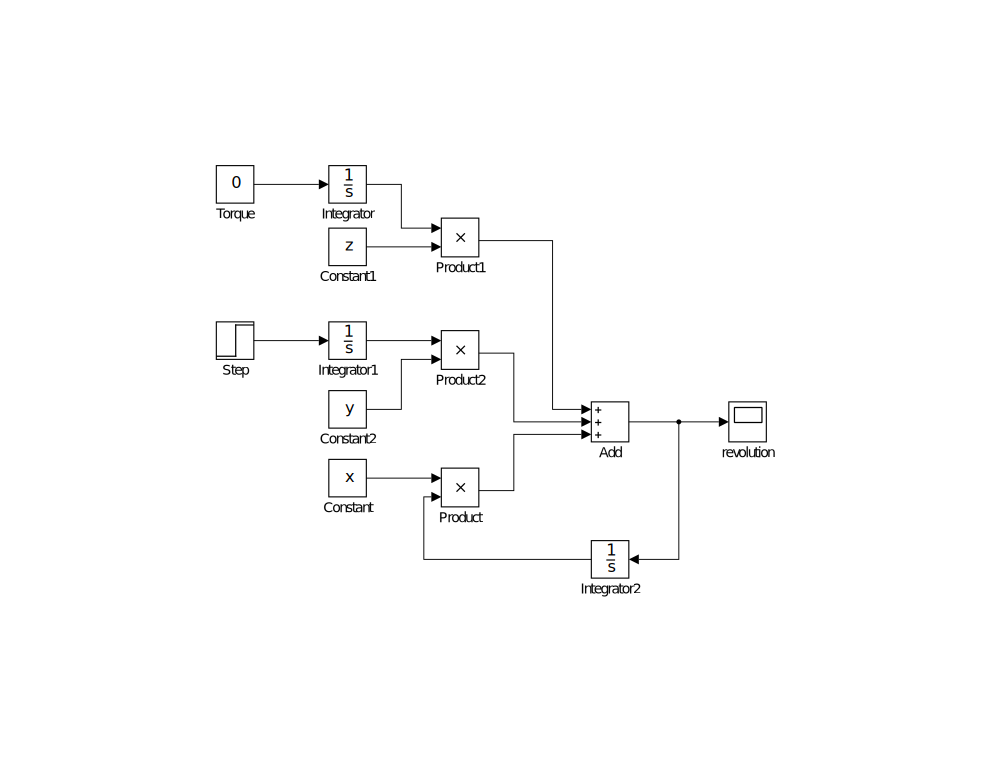
\includegraphics[width=1\textwidth]{../../matlab/exercise/ex_01/ex_01.pdf}
	\caption{Simulink-Model}
\end{figure}

\subsection{Plausibilitätsprüfung}
Um die plausibilität des Modells zu prüfen weden spezifische Zustände geprüft.

\subsubsection{Unbelastete Welle}
Wird der Motor mit positiver Spannung und ohne Lastmoment betireben, so muss
sich eine positive Drehzahl einstellen. Die Motorspannung ist mit einer
Sprungfunktion gegeben mit der Amplitude 1. Die Simulation zeigt, dass sich
eine Drehzahl von 5 einstellt.

\subsubsection{Belastete Welle}
Liegt ein positives Lastmoment an, wobei keine Spannung anliegt, so muss sich
eine negative Drehzahl einstellen. Für diese Prüfung ist ein Lastmoment
$\Gamma(t) = const. = 1$ gewählt worden. Die Simulation zeigt, dass sich eine
Drehzahl von -0.5 einstellt.

\subsection{Überbelastete Welle}
Wird der Motor mit einem grossen Lastmoment belastet, so muss sich eine
negative Drehzahl einstellen. Das Lastmoment ist konstant gewählt als
$\Gamma(t) = const. = 10$ und die Motorspannung ist als Sprungfunktion
gegeben mit der Amplitude 5. Die Simulation zeigt, dass sich vor dem Sprung
eine Drehazhl von -5 einstellt durch das Lastmoment. Nach den Sprung
resultiert eine Drehzahl von -2.5 durch das entgegenwirken des Motors.

\subsubsection{Anfangsbedingung $\omega(t=0) \neq 0$}
Liegt weder ein Lastmoment an der Welle noch eine Spannung am Motor, so muss
sich die Drehzahl für die Anfangsbedingung $\omega(t=0) \neq 0$ gegen 0
annähern. Die Simulation zeigt, dass sich die Drehzahl gegen 0 annähert mit
der Zeit. Dies gilt sowohl für positive als auch negative Anfangsbedingungen.

\subsubsection{Sinus als Eingangsfunktion}
Wird eine Sinusfunktion für die Motorspannung gewählt, so muss sich auch
eine Sinusgrösse am Ausgang einstellen. Dies muss für jedes anliegende
Lastmoment an der Welle gelten. Die Simulationen haben gezeigt, dass sich
für alle Lastmomente eine Sinusförmige Drehzahl ergibt für eine Sinusförmige
Motorspannung. der Offset der Sinuskurve am Ausgang ist dabei gegeben durch
das anliegenede Lastmoment.

\subsubsection{Fazit}
Die Plausibilitätsprüfungen deuten darauf hin, dass das modellierte System
sich wie erwartet verhält.
		\newpage	% Wirkungsplan
\section{Übertragungsfunktionen}

\subsection{$P_1(s)$}
Die Übertragungsfunktion $P_1(s)$ ist gegeben als
\[
	P_1(s) = \frac{\Omega(s)}{U(s)}
\]
Um diese Übertragungsfunktion herzuleiten muss die ursprüngliche
Differetialgleichung betrachtet werden.
\[
	\dot\omega(t) = x \omega(t) + y u(t) + z \Gamma(t)
\]
Da für diese Übertragungsfunktion $\omega(t)$ von Interesse ist, kann die
Funktion dementsprechend in die explizite Form für $\omega(t)$ umgeformt
werden. Dies ist mittels der Integration nach der Zeit $t$ zu bewerkstelligen.
\[
	\omega(t) =
		x \int\omega(t)\,dt
		+ y \int U(t)\,dt 
		+ z \int\Gamma(t)\,dt
\]
Um nun diese Differetialgleichung in den Spektralbereich zu überführen,
können der Linearitätssatz und der Integrationssatz der Laplace-Transformation
genutzt werden.
\[
	\Omega(s) =
		x \frac{1}{s} \Omega(s) 
		+ y \frac{1}{s} U(s)
		+ z \frac{1}{s} \Gamma(s) 
\]
Die nun vorliegende Gleichung im Spektralbereich ist so umzuformen, dass diese
als Qoutient von Ein- und Ausgangsgrösse dargestellt werden kann. In einem
ersten Schritt sind die entsprechenden Termen zu faktorisieren.
\[
	\Omega(s) - x \frac{1}{s} \Omega(s) =
		y \frac{1}{s} U(s) + z \frac{1}{s} \Gamma(s)
\]
\[
	\Omega(s) \left[ 1 - x \frac{1}{s} \right] =
		U(s) \left[ y \frac{1}{s} \right]
		+ \Gamma(s) \left[ z \frac{1}{s}\right]
\]
Betrachtet man die nun vorliegende Gleichung, so stellt man fest, dass eine
Summe vorliegt welche die Bildung des gewünschten Quotienten verhindert.
Betrachtet man diese Gleichung genauer und führt eine Identifikation durch, so
stellt sich heraus, dass einer der Summanden nicht zum relevanten Signalpfad
gehört. Somit kann dieser Teil der Gleichung gestrichen werden
(``\emph{single input, single output}'').
\[
	\underbrace{\Omega(s) \left[ 1 - x \frac{1}{s} \right]}_{Ausgang} =
		\underbrace{U(s) \left[ y \frac{1}{s} \right]}_{Eingang 1}
		+ \underbrace{\Gamma(s) \left[ z \frac{1}{s}\right]}_{Eingang 2}
	\qquad \Gamma(s) = 0 \Rightarrow
		\Omega(s) \left[ 1 - x \frac{1}{s} \right] =
		U(s) \left[ y \frac{1}{s} \right]
\]
Mit dieser Reduktion lässt sich nun die Übertragungsfunktion $P_1(s)$
formulieren.
\[
	P_1(s) = \frac{\Omega(s)}{U(s)} =
		\frac{y \frac{1}{s}}{1 - x \frac{1}{s}} = 
		\frac{\frac{1}{s} y}{\frac{1}{s} (s-x)} =
		\frac{y}{s-x}
\]

\subsection{$P_2(s)$}
Die Übertragungsfunktion $P_2(s)$ ist gegeben als
\[
	P_2(s) = \frac{\Omega(s)}{\Gamma(s)}
\]
Um diese Übertragungsfunktion herzuleiten muss die ursprüngliche
Differetialgleichung betrachtet werden.
\[
	\dot\omega(t) = x \omega(t) + y u(t) + z \Gamma(t)
\]
Da für die Übertragungsfunktion $\Gamma(t)$ von Interesse ist, kann die
Funktion dementsprechend in die explizite Form für $\Gamma(t)$ umgeformt
werden.
\[
	\Gamma(t) = \frac{1}{z} \left(
			\dot\omega(t) - x \omega(t) - y u(t)
		\right)
\]
Um nun diese Differetialgleichung in den Spektralbereich zu überführen, kann
der Linearitätssatz und der Differentiationssatz der Laplace-Transformation
verwendet werden.
\[
	\Gamma(s) = \frac{1}{z} \left(
			s \Omega(s) - \omega(0^-) - x \Omega(s) - y U(s)
		\right)
\]
Die nun vorliegende Gleichung im Spektralbereich ist so umzuformen, dass diese
als Quotient von Ein- und Ausgangsgrösse dargestellt werden kann.
\[
	\Gamma(s) = \frac{1}{z} \left(
			\Omega(s) \left[ s-x \right] - \omega(0^-) - y U(s)
		\right)
\]
Betrachtet man die nun vorliegende Gleichung, so stellt man fest, dass eine
Summe vorliegt welche die Bildung des gewünschten Quotienten verhindert.
Betrachtet man diese Gleichung genauer und führt eine Identifikation durch, so
stellt sich heraus, dass einer der Summanden nicht zum relevanten Signalpfad
gerhört. Somit kann dieser Teil der Gleichung gestrichen werden. Weiter ist
zu erkennen, dass eine Anfangsbedingung vorliegt, welche man auch voraussetzen
kann mit 0.
\[
	\underbrace{\Gamma(s)}_{Eingang 1} = \frac{1}{z} \left(
			\underbrace{\Omega(s) \left[ s-x \right]}_{Ausgang}
			\underbrace{- \omega(0^-)}_{\begin{subarray}{c}Anfangs-\\ bedingung\end{subarray}}
			\underbrace{- y U(s)}_{Eingang 2}
		\right)
	\qquad U(s) = \omega(0^-) = 0 \Rightarrow \Gamma(s) =
		\frac{1}{z} \left[ s-x \right]
\]
Mit dieser Reduktion lässt sich nun die Übertragungsfunktion $P_2(s)$
formulieren.
\[
	P_2(s) = \frac{\Omega(s)}{\Gamma(s)} = \frac{z}{s-x}
\]
		\newpage	% Übertragungsfunktion
\section{Übertragungsfunktionen programmieren}
\begin{figure}[h!]
	\centering
	\includegraphics[width=1\textwidth]{../../matlab/exercise/ex_03/ex_03_model.pdf}
	\caption{Simulink-Modell}
\end{figure}
		\newpage	% TRF programmieren
\section{Bode-Diagramm von $P_1(s)$}
\begin{figure}[h!]
	\centering
	\includegraphics[scale=1]{../../matlab/exercise/ex_04/ex_04_model.pdf}
	\caption{Simulink-Modell}
\end{figure}

\subsection{Betrachtung der Übertragungsfunktion $P_1(s)$}
Die vorliegende Übertragungsfunktion 
\[
	P_1(s) = \frac{y}{s-x} = \frac{400}{s - (-20.4)} = \frac{400}{s + 20.4}
\]
kann normiert werden, so dass ein typisches PT$_1$-Glied daraus resultiert.
\[
	P_1(s) = \frac{400}{s + 20.4}
		\frac{\left(\frac{400}{20.4}\right)}{1 + \left(\frac{1}{20.4}\right)s}
		\Leftrightarrow \frac{k_p}{1 + T_1 s}
\]
Die Eckwerte eines solchen PT$_1$-Gliedes sind
\begin{itemize}
	\item $|G_0| = 20 \log (kp) = 25.85\mathrm{dB}$
	\item $\omega_0 = \omega(G = G_0 - 3\mathrm{dB}) = \frac{1}{T_1} = 20.4$
	\item $\varphi(\lim_{\omega \rightarrow 0}) = 0^{\circ}$, 
		$\varphi({\omega(G = G_0 - 3\mathrm{dB})}) = -45^{\circ}$,
		$\varphi(\lim_{\omega \rightarrow \infty}) = -90^{\circ}$
	\item $-20\frac{\mathrm{dB}}{\mathrm{Dekade}}$ ab $\omega_0$
\end{itemize}
Das exakte Bodediagramm dieses Übertragungsgliedes ist in der Abbildung
\ref{fig:bode_p1} dargestellt.
\begin{figure}[h!]
	\centering
	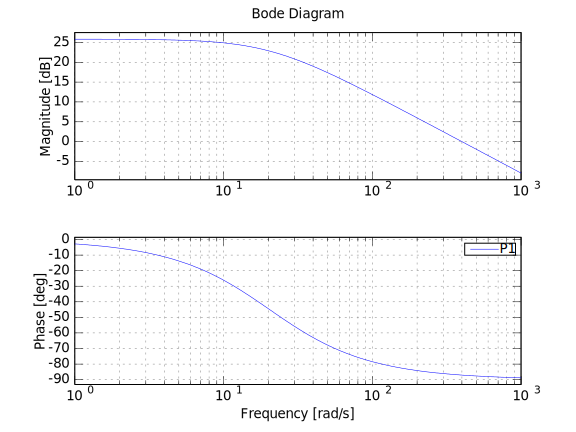
\includegraphics[width=1\textwidth]{../../matlab/exercise/ex_04/bode_p1.pdf}
	\caption{Bode-Diagramm von $P_1(s)$}
	\label{fig:bode_p1}
\end{figure}
		\clearpage	% Bode P1(s)
\section{Bode-Plot mit HSLU-Script
		\newpage	% Nyquist P1(s)
\section{MATLAB Skript}
		\clearpage	% asymp
\section{Steuerung}

\subsection{Blockschaltbild}

\begin{figure}[h!]
	\centering
	\begin{tikzpicture}[node distance=2cm]
		% nodes
		\node [input] (in1) {};
		\node [function, right of=in1] (st) {$S_t$};
		\node [function, right of=st] (p1) {$P_1$};
		\node [sum, right of=p1] (sum) {$\Sigma$};
		\node [function, above of=p1] (p2) {$P_2$};
		\node [input, left of=p2] (in2) {};
		\node [output, right of=sum] (out) {};
		% arrows
		\draw[->] (in1) node[anchor=east] {$\Omega_r$} -- (st);
		\draw[->] (in2) node[anchor=east] {$\Gamma$} -- (p2);
		\draw[->] (st) -- (p1);
		\draw[->] (p1) -- (sum);
		\draw[->] (p2) -| (sum);
		\draw[->] (sum) -- (out) node[anchor=west] {$\Omega$};
		% legend
	\end{tikzpicture}
	\caption{Blockschaltbild der Drehzahlsteuerung (``\emph{open loop}'')}
\end{figure}
		\newpage	% Blockschaltbild
\section{Steuerung programmiren in MATLAB}
		\newpage	% Steuerung
\section{Regler}

\subsection{Blockschaltbild}

\begin{figure}[h!]
	\centering
	\begin{tikzpicture}[node distance=2cm]
		% nodes
		\node [input] (in0) {};
		\node [sum, right of=in0] (in1) {$\Sigma$};
		\node [function, right of=in1] (c) {$C$};
		\node [function, right of=c] (p1) {$P_1$};
		\node [sum, right of=p1] (sum) {$\Sigma$};
		\node [function, above of=p1] (p2) {$P_2$};
		\node [input, left of=p2] (in2) {};
		\node [dot, right of=sum] (out1) {};
		\node [output, right of=out1] (out2) {};
		\node [output, below of=out1] (out3) {};
		% arrows
		\draw[->] (in0) node[anchor=east] {$\Omega_r$} -- (in1);
		\draw[->] (in1) -- (c);
		\draw[->] (in2) node[anchor=east] {$\Gamma$} -- (p2);
		\draw[->] (c) -- (p1);
		\draw[->] (p1) -- (sum);
		\draw[->] (p2) -| (sum);
		\draw[->] (sum) -- (out2) node[anchor=west] {$\Omega$};
		\draw[->] (out1) |- (out3) -| (in1);
		% legend
	\end{tikzpicture}
	\caption{Blockschaltbild der Drehzahlregelung (``\emph{closed loop}'')}
\end{figure}
		\newpage	% Regler
\section{Übertragungsfunktion des offene Regelkreises}
Der Reglekreis hat zwei Eingänge. An einem der Eingänge liegt die
Referenzdrehzahl $\omega_r$ an. Der andere Eingang dient der Störgrösse
$\Gamma$ und ist nicht von der Referenzdrehzahl abhängig. Somit lässt
sich der Offene Reglekreis formulieren aus der Summe dieser zwei Signalpfade
welche überlagert am Ausgang anliegen.
\[
	\omega = \omega_r \cdot L(s) + \Gamma \cdot P_2(s)
\]
Die Übertragungsfunktion des Pfades welcher vom Eingang mit der Referenzdrehzahl
zum Ausgang führt, kann somit isoliert betrachtet werden.
\[
	L(s) = C(s) \cdot P_1(s) = C(s) \cdot \frac{y}{s-x}	
\]
		\newpage	% offener Regelkreis
\section{Offener Regelkreis}
		\newpage	% Reglertyp
\section{Gliedidentifikation}
		\newpage	% Übertragungsfunktion
\section{Stabilitätsreserve}
Für das Bestimmen der Stabilitätsreserve sollen zwei Wertebereiche für den
Regler gewählt werden.
\[
	K_p  = \left\{
		\begin{array}{l}
			K_p < \frac{1}{K_g} \\
			K_p > \frac{1}{K_g}
		\end{array}
	\right.
\]
Für diese Aufgabe wird angenommen, dass $K_g$ den Proportionalanteil
der normierten Übertragungsfunktion der Stecke darstellt.
\[
	K_g = \frac{y}{x} = \frac{K}{K^2 + \alpha R}
\]
Da keine expliziten Werte gegeben sind, wird zunächt der Grenzfall
betrachtet mit
\[
	K_p = \frac{1}{K_g} = \frac{K^2 + \alpha R}{K}
\]
Die Übertragungsfunktion für den relevanten Signalpfad ergibt sich somit zu
\[
	L(s) = \frac{1}{K_g} \cdot \frac{K_g}{1 + T_1 \cdot s}
	= \frac{1}{1 + T_1 \cdot s} 
	= \frac{1}{1 + \frac{1}{\frac{1}{J} \cdot \left(
		\alpha + \frac{K^2}{R} \right) } \cdot s }
\]
Das daraus resultierende Glied stellt einen Tiefpass dar (PT$_1$-Glied).
Dieses hat einen resultierenden Proportionalitätsfaktor von 0, da der 
Regler $K_g$ reziprok als Faktor inplementiert. Somit ergibt sich der
Verlauf eines Tiefpasses mit $G_0 = 0$. Eine Skalierung beim Regler
verändert das Verhalten der Übertragung in der Weise, dass legiglich die
DC-Verstärkung abgehiben oder abgesenkt wird. Dies ist in der Abbildung
\ref{fig:ex_13_bode} dargestellt.
\begin{figure}[h!]
	\centering
	\includegraphics[width=\textwidth]{../../matlab/exercise/ex_13/ex_13_bode.pdf}
	\caption{Bode-Diagramm des Grenzfalls}
	\label{fig:ex_13_bode}
\end{figure}
Die Stabilitätsreserven (Amplitudenreserve $A_R$ und Phasenreserve
$\varphi_R$) sind dirket deutbar aus dem Plot \ref{fig:ex_13_bode}.

\subsection{Grenzfall $K_p = {K_g}^{-1}$}
Für den Grenzfall wird deutlich, dass der Durchtritt ($G = 0$dB) schon
bei einer Phasenverschiebung von $\varphi > 0^{\circ}$ erfolgt.
Da es sich um einen einfachen Tiefpass (Tiefpass erster Ordnung bzw.
PT$_1$-Glied) handelt, wird dessen Phase
asymptotisch gegen $-90^{\circ}$ gehen. Somit ergibt sich eine unendliche
Amplitudenreserve $A_R = \infty$. Die Phasenreserve ist dabei exakt
$\varphi_R = 180^{\circ}$, da der Durchtritt bereits bei
$\varphi > 0^{\circ}$ erfolgt.

\subsection{$K_p > {K_g}^{-1}$}

\subsection{$K_p < {K_g}^{-1}$}

\subsection{MATLAB Script und Ergebnisse}

\lstinputlisting{../../matlab/exercise/ex_13/ex_13_init.m}
\lstinputlisting{../../matlab/exercise/ex_13/ex_13_bode.m}
\lstinputlisting{../../matlab/exercise/ex_13/results.txt}

		\clearpage	% Stabilitätsreserve
\section{Geschlossener Regelkreis}

\subsection{Führungsübertragungsfunktion $G_F(s)$}
Die Führungsübertragungsfunktion setzt sich zusammen aus dem
direkten Signalpfad von Eingang zu Ausgang des Systems und dem
Kreispfad.
\[
	G_F(s) = \frac{C(s) \cdot P_1(s)}{1 + C(s) \cdot P_1(s)}
\]
Resubstituiert man die einzelnen Glieder mit ihren normierten Komponenten
so ergibt sich die explizite Führungsübertragungsfunktion.
\[
	G_F(s)
	= \frac{C(s) \cdot P_1(s)}{1 + C(s) \cdot P_1(s)}
	= \frac{
		K_p \cdot \frac{K_{g_1}}{1+T_1\cdot s}
	}{
		1 + K_p \cdot \frac{K_{g_1}}{1+T_1\cdot s}	
	}
	= \frac{K_p \cdot K_{g_1}}{1 + T_1 \cdot s + K_p \cdot K_{g_1}}
\]

\subsection{Störübertragungsfunktion $G_S(s)$}
Die Störübertragungsfunktion setzt sich zusammen aus dem direkten Pfad
von der Störquelle hin zum Ausgang (denn ein Kreispfad ist im vorliegenden
Modell nicht vorhanden).
\[
	G_S(s) = P_2(s)
\]
Resubstituiert man die Übertragungsfunktion $P_2(s)$ mit den normierten
Komponenten so ergibt sich die explizite Störübertragungsfunktion.
\[
	G_S(s) = P_2(s) = \frac{z}{s-x} = \frac{K_{g_2}}{1 + T_2 \cdot s}
\]
		\newpage	% Geschlossener Regelkreis
\section{Geschlossener Regelkreis}
		\newpage	% Simulink closed loop
\section{Stationäre Regeldifferenz}
Die stationäre Regeldifferenz lässt sich mittels des Endwertsatzes von
Laplace ermitteln.
\[
	\omega(\infty)
	= \lim_{s \rightarrow 0} s \cdot G_F(s) \cdot \Omega(s)	
\]
Hierbei ist $G_F(s)$ die Führungsübertragungsfunktion und $\Omega(s)$ die
Laplace-Transformierte des Eingangssignals. Dieses soll hier als
Einheitssprung mit der Amplitude 1 gegeben sein.
\[
	\omega(t)
	= 1 \cdot \sigma(t) \quad \laplace \quad \Omega(s) = \frac{1}{s}
\]
Wendet man den Endwertsatz an auf die gegebenen Funktionen so ergibt sich
\[
	\omega(\infty)
	= \lim_{s \rightarrow 0} s \cdot G_F(s) \cdot \Omega(s)	
	= s \cdot \frac{
		K_p \cdot K_{g_1}
	}{
		1 + T_1 \cdot s + K_p + K_{g_1}
	} \cdot \frac{1}{s}
	= \frac{K_p \cdot K_{g_1}}{1 + K_p \cdot K_{g_1}}
\]
Nun wird deutlich, dass die Regeldifferenz direkt von der Auslegung der
Propotionalitätskonstante $K_p$ des Reglers abhängt. Wählt man beispielsweise
ein $K_p$, so dass dieses dem reziproken Wert des $K_{g_1}$ entspricht, so
ergibt sich ein Propotionalitätfaktor von $K_p \cdot K_{g_1} = 1$. Setzt man
dies ein, so ergibt sich ein Endwert von 
\[
	\omega(\infty) = \frac{1}{1+1} = \frac{1}{2} = 0.5 = 50\%	
\]
Wird das $K_p$ hingegen kleiner ${K_{g_1}}^{-1}$ gewählt, so wird der Endwert
nochmals kleiner als bei der Gleichheit.
\[
	K_p < \frac{1}{K_{g_1}}
	\Rightarrow K_p \cdot K_{g_1} < 1 
		\Rightarrow \omega(\infty) \xrightarrow{K_p \rightarrow 0} 0
\]
Wird das $K_p$ hingegen grösser gewählt, so wird der Endwert höher.
\[
	K_p > \frac{1}{K_{g_1}}
	\Rightarrow K_p \cdot K_{g_1} > 1
		\Rightarrow \omega(\infty) \xrightarrow{K_p \rightarrow \infty} 1
\]

\subsection{Prüdung der Endwerte mit MATLAB/Simulink}
Die Simulation des Systems mit Simulink bestätigt die Annahmen, welche sich
durch den Endwertsatz ergeben.

\begin{figure}[h!]
	\centering
	\includegraphics[width=1\textwidth]{../../matlab/exercise/ex_16/ex_16_plot.pdf}
	\caption{Endwerte zum Einheitssprung bei unterschiedlichen $K_p$}
\end{figure}
		\newpage	% Endwertsatz
\section{Reglerauslegung}
Die Auslegung des Proportionalitätsfaktors $K_p$ des Reglers, unter
Berücksichtigung der Stabilitätsanalyse und des stationären Regelfehlers,
sollte nach Möglichkeit hoch ausfallen. Dies beweikt, dass der stationäre
Regelfehler gegen 0 strebt. Die Stabilität ist hiervon nicht tangiert
(vorausgesetzt das Lastmoment ist $\Gamma = 0$).

Wird ein Lastmoment $\Gamma \neq 0$ angelegt, so gilt die obige aussage
nicht. Denn der Einfluss der Störgrösse wird überlagert auf die
Ausgangsgrösse. Je höher der Proportionalitätsfaktor gewählt wird, desto
höher ist die Schwingneigung. 

Simulationen mit dem Modell in MATLAB/Simulink zeigen, dass sich mit einem
hohen $K_p$ und einem $\Gamma \neq 0$ nie ein stationärer Wert am Ausgang
einstellt bei konstanter Führungsgrösse. Wählt man das $K_p$ jedoch kleiner,
so wird die Amplitude und Frequenz der Schwingungen heruntergesetzt.

Betrachtet man die Störübertragungsfunktion im Bode-Diagramm (siehe Abbildung
\ref{fig:ex_17_bode_p2}), so erkennt man, dass dort eine massive
DC-Verstärkung $G_0 > 45$dB vorliegt. Zuden ist zu erkennen, dass die
Phase nicht bei $0^{\circ}$ beginnt, sondern bei $180^{\circ}$. Dies ist so,
da die Störung sich negativ, also der Drehzahl $\omega$ entgegenwikrt.

\begin{figure}[h!]
	\centering
	\includegraphics[width=1\textwidth]{../../matlab/exercise/ex_17/ex_17_bode_p2.pdf}
	\caption{Bode-Diagramm der Störübertragungsfunktion $P_2(s)$}
	\label{fig:ex_17_bode_p2}
\end{figure}
		\newpage	% Auslegung
\section{Regleridentifikation}
Der Regler sei gegeben als
\[
	C(s) := K(s) = K_p \left( 1 + \frac{1}{T_i s} \right)
	= \underbrace{K_p}_{P} + \underbrace{\frac{K_p}{T_i} \cdot \frac{1}{s}}_{I}
	= K_p \left( \frac{T_i s}{T_i s} + \frac{1}{T_i s} \right)
	= K_p \left( \frac{T_i s + 1}{T_i s} \right)
\]
Deutlich zu erkennen sind dabei der Proportionalanteil und der Integralanteil
der Übertragungsfunktion. Es handelt sich hier eindeutig um einen PI-Regler.
Isoliert man die beiden Anteile, so ergeben sich die Funktionen
\[
	I: \qquad \frac{K_p}{T_i} \cdot \frac{1}{s} 
	= X(s) \cdot \frac{1}{s}
		\quad \Laplace
		\quad \frac{K_p}{T_i} \int_{0^-}^{t} x(t)\,dt
\]
\[
	P: \qquad K_p
\]
wobei $x(t)$, $X(s)$ die Eingangsgrösse beschreibt. 
		\newpage	% Regleridentifikation
\section{Parameter des PI-Reglers}
Für die Betrachtung des offenen Regelkreises mit dem PI-Regler wird dieser
in einem ersten Schritt für den Grenzfall $T_i = \tau_g$ ausgelegt.
\[
	\tau_g := \frac{J R}{K^2 + \alpha R} \approx 0.05 
\]
Somit ergibt sich die folgende Übertragungsfunktion für den offenen
Regelkreis.
\[
	L(s)
	= C(s) \cdot P_1(s)
	= K_p \cdot \left(
		1 + \frac{1}{T_i s}
	\right) \cdot \left(
		\frac{y}{s-x}
	\right)
	= \underbrace{\left(
		K_p + \frac{
			K_p \left(K^2 + \alpha R\right)
		}{JR} \cdot \frac{1}{s}
	\right)}_{\text{PI-Regler}} \cdot \underbrace{\left(
		\frac{
			\frac{K}{R \left(\alpha + \frac{K^2}{R}\right)}
		}{
			1 + \frac{J}{\alpha + \frac{K^2}{R}} \cdot s
		}
	\right)}_{\text{PT$_1$-Strecke}}
\]
Aus der oben aufgeführten Übertragungsfunktion $L(s)$ lassen sich nun
direkt die Kennwerte für das Bode-Diagramm auslesen. Der Durchtrittspunkt
$\omega_D$ ist gegeben durch den Faktor zum Integralanteil $s^{-1}$.
\[
	\text{I}: \qquad \underbrace{k_i}_{\omega_D} \cdot \frac{1}{s}
\]
Dieser ist aus obiger Übertragungsfunktion direkt auszulesen.
\[
	L(s) = \left(
		K_p + \underbrace{\frac{
			K_p \left(K^2 + \alpha R\right)}{JR}}_{\omega_D}
		\cdot \frac{1}{s}
	\right) \cdot \left(
		\frac{
			\frac{K}{R \left(\alpha + \frac{K^2}{R}\right)}
		}{
			1 + \frac{J}{\alpha + \frac{K^2}{R}} \cdot s
		}
	\right)
\]
Der Summand $K_p$ bildet dabei lediglich die Limitierung für die Dämpfung.
D.h., dass die Verstärkung asymtotisch zu 0 geht statt logarithmisch (linear
im Bode-Diagramm mit logarithmischer Darstellung) nach $\infty$, wie dies
beim idealen Integrator der Fall ist (hier liegt ein PI-Glied vor).
Dieser P-Anteil bewirkt auch eine Phasenhebung von $+90^{\circ}$ (ausgehend
von $-90^{\circ}$ für $\omega \rightarrow 0$ hervorgerufen durch den
Integrator). Die Bode-Diagramme für diese Auslegung sind in der Abbildung
\ref{fig:ex_19_bode_border} dargestellt. In dieser Abbildung ist deutlich
zu erkennen, dass sich die Phasenhebung des PI-Gliedes und die Phasensenkung
des PT$_1$-Gliedes gegenseitig aufheben, so dass eine Phase von
$\varphi = 90^{\circ}$ reusltiert. Auch der Amplitudengang wird durch die
Kombination von PI- und PT$_1$-Glied so verändert, dass ein Amplitudengang
eines idealen Integrators resultiert. Die Abbildung
\ref{fig:ex_19_bode_variants} zeigt den Einfluss der Auslegung von $T_i$
im Verhältnis zu $\tau_g$.

\begin{figure}[h!]
	\centering
	\includegraphics[width=1\textwidth]{../../matlab/exercise/ex_19/ex_19_bode.pdf}
	\caption{Bode-Diagramm des Reglers $C(s)$, der Strecke $P_1(s)$ und des
		direkten Signalpfades $L(s)$.}
	\label{fig:ex_19_bode_border}
\end{figure}

\begin{figure}[h!]
	\centering
	\includegraphics[width=1\textwidth]{../../matlab/exercise/ex_19/ex_19_bode_02.pdf}
	\caption{Bode-Diagramm von $L(s)$ für $T_i = \tau_g$,
		$T_i > \tau_g$, $T_i < \tau_g$.}
	\label{fig:ex_19_bode_variants}
\end{figure}
		\clearpage	% Parameter des PI-Reglers
\section{Vereinfachung}
		\newpage	% Grenzfall
\section{Stabilitätsreserve}
		\newpage	% Stabilität
\section{MATLAB/Simulink Modell des PI-Reglers}

\lstinputlisting{../../matlab/exercise/ex_22/ex_22_init.m}

\begin{figure}[h!]
	\centering
	\includegraphics[scale=1]{../../matlab/exercise/ex_22/ex_22_model.pdf}
	\caption{Simulink-Modell des PI-Reglers}
	\label{fig:ex_22_model}
\end{figure}
		\newpage	% PI-Regler im Simulink
%\section{Stationäre Regeldifferenz des PI-Reglers}
Um die stationäre Regeldifferenz zu ermitteln, muss zunächst die
Übertragungsfunktion formuliert werden.
\[
	G_F(s) = \frac{G_0(s)}{1+G_0(s)}
\]
Die \emph{open-loop}-Übertragungsfunktion $G_0(s)$ ist gegeben als
\[
	G_0(s)
	= C(s) \cdot P_1(s)
	= K_p \left( 1 + \frac{1}{T_i s} \right) \frac{y}{s-x}
	= \frac{K_p(T_i s + 1) y}{T_i s (s-x)}
\]
Mit dieser lässt sich nun die \emph{closed-loop}-Übertragungsfunktion
formulieren zu
\[
	G_F(s)
	= \frac{G_0(s)}{1 + G_0(s)}
	= \frac{
		\left( \frac{K_p(T_i s + 1) y}{T_i s (s-x)} \right)
	}{
		1 + \left( \frac{K_p(T_i s + 1) y}{T_i s (s-x)} \right)
	}
	= \frac{
		K_p y (T_i s + 1)
	}{
		T_i(s^2 - sx) + K_p y (T_i s + 1)
	}
\]
Für die Anwendung des Endwertsatzes der Laplace-Transformation ist das
Eingangssignal angenommen als Einheitssprung mit der Amplitude 1.
\[
	\omega(\infty)
	= \lim_{s \rightarrow 0} \left(
		\underbrace{s \cdot \Omega(s)}_{1} \cdot G_F(s)
	\right)
	= \lim_{s \rightarrow 0} G_F(s)
	= K_p \cdot y \cdot \lim_{s \rightarrow 0} \left(
		\frac{
			\overbrace{T_i s}^{0} + 1
		}{
			\underbrace{T_i(s^2 - sx)}_{0} 
			+ \underbrace{K_p y (T_i s + 1)}_{K_p y}
		}
	\right)
	= 1
\]
Der Endwert entspricht also zu 100\% der Eingangsgrösse, somit existiert
kein stationäre Regelfehler.
		\newpage
%\section{Signalbegrenzung}

\subsection{MATLAB/Simulink-Modell}

\begin{figure}[h!]
	\centering
	\includegraphics[width=1\textwidth]{../../matlab/exercise/ex_24/ex_24_model.pdf}
	\caption{Simulink-Modell des geregelten Motors mit Signalbegrenzung}
\end{figure}

\subsection{Simulationsergebnisse}
Je niedriger $K_p$ gewählt wird, desto träger ist der Ausgleichsvorgang.
Die Drehzahl reagiert mit einer $e$-Kurve auf einen Sprung. Rippel oder
Schwingungen auf der Drehzahl sind jedoch keine vorhanden. Auch bei der
Eingangsspannung des Motors ist keinerlei Rippel zu beobachten.

Wählt man aber ein hohes $K_p$, so ist der Ausgleichsvorgang eher linear.
Bei sehr hohem $K_p$ zeigt die Spannung am Motoreneingang dann jedoch
dutliche Rippel bzw. Schwingungen auf.

\begin{figure}[h!]
	\centering
	\begin{subfigure}{0.45\textwidth}
		\includegraphics[width=1\textwidth]{../../matlab/exercise/ex_24/ex_24_01.pdf}
		\caption{$u(t)$ und $\omega(t)$ bei kleinem $K_p$}
	\end{subfigure}
	\hfill{}
	\begin{subfigure}{0.45\textwidth}
		\includegraphics[width=1\textwidth]{../../matlab/exercise/ex_24/ex_24_02.pdf}
		\caption{$u(t)$ und $\omega(t)$ bei grossen $K_p$}
	\end{subfigure}
	\caption{Simulationen verschiedener $K_p$}
\end{figure}
		\newpage
%\section{Signalbegrenzung - Integrator}

\subsection{MATLAB/Simulink-Modell}

\begin{figure}[h!]
	\centering
	\includegraphics[width=1\textwidth]{../../matlab/exercise/ex_25/ex_25_model.pdf}
	\caption{Simulink-Modell des geregelten Motors mit Signalbegrenzung}
\end{figure}

\subsection{Simulationsergebnisse}
\begin{figure}[h!]
	\centering
	\begin{subfigure}{0.45\textwidth}
		\includegraphics[width=1\textwidth]{../../matlab/exercise/ex_25/ex_25_01.pdf}
		\caption{Sprungantwort für kleines $K_p$}
		\label{fig:ex_25_01}
	\end{subfigure}
	\hfill{}
	\begin{subfigure}{0.45\textwidth}
		\includegraphics[width=1\textwidth]{../../matlab/exercise/ex_25/ex_25_02.pdf}
		\caption{Sprungantwort für grosses $K_p$}
	\end{subfigure}
	\caption{Simulation der Sprungantworten mit verschienenen $K_p$}
\end{figure}

\begin{figure}[h!]
	\centering
	\begin{subfigure}{0.45\textwidth}
		\includegraphics[width=1\textwidth]{../../matlab/exercise/ex_25/ex_25_11.pdf}
		\caption{Impulsantwort für kleines $K_p$}
		\label{fig:ex_25_11}
	\end{subfigure}
	\hfill{}
	\begin{subfigure}{0.45\textwidth}
		\includegraphics[width=1\textwidth]{../../matlab/exercise/ex_25/ex_25_12.pdf}
		\caption{Impulsantwort für grosses $K_p$}
	\end{subfigure}
	\caption{Simulation der Impulsantworten mit verschiedenen $K_p$}
\end{figure}
		\newpage
%\section{Signalbegrenzung - Anti-Windup}

\subsection{MATLAB/Simulink-Modell}

\begin{figure}[h!]
	\centering
	\includegraphics[width=1\textwidth]{../../matlab/exercise/ex_26/ex_26_model.pdf}
	\caption{Simulink-Modell des geregelten Motors mit Signalbegrenzung
		und Anti-Windup}
\end{figure}

\subsection{Simulationsergebnisse}
\begin{figure}[h!]
	\centering
	\begin{subfigure}{0.45\textwidth}
		\includegraphics[width=1\textwidth]{../../matlab/exercise/ex_26/ex_26_01.pdf}
		\caption{Sprungantwort für kleines $K_p$}
	\end{subfigure}
	\hfill{}
	\begin{subfigure}{0.45\textwidth}
		\includegraphics[width=1\textwidth]{../../matlab/exercise/ex_26/ex_26_02.pdf}
		\caption{Sprungantwort für grosses $K_p$}
	\end{subfigure}

	\begin{subfigure}{0.45\textwidth}
		\includegraphics[width=1\textwidth]{../../matlab/exercise/ex_26/ex_26_11.pdf}
		\caption{Störverhalten für kleines $K_p$}
	\end{subfigure}
	\hfill{}
	\begin{subfigure}{0.45\textwidth}
		\includegraphics[width=1\textwidth]{../../matlab/exercise/ex_26/ex_26_12.pdf}
		\caption{Störverhalten für grosses $K_p$}
	\end{subfigure}

	\caption{Simulationen verschiedener $K_p$ für das Anti-Windup}

\end{figure}
		\newpage
%\section{Vorsteuerung $F(s)$}

\begin{figure}[h!]
	\centering
	\includegraphics[width=0.75\textwidth]{fig/ex_27_cs.pdf}
\end{figure}
		\newpage
%\section{Analyse der Vorsteuerung}
		\newpage

% appendix
\clearpage
\begin{appendices}
	\clearpage
	\pagenumbering{roman}
	\section{Aufgabenstellung}

\includepdf[pages=-,offset=0 -2.2cm,frame,width=0.92\textwidth,picturecommand={\centering},pagecommand={\thispagestyle{fancy}},]{bin/RTL_VorbereitungUebung.pdf}

\end{appendices}

